% CANONICAL_AAAI_SUBMISSION_SOURCE
% This is the authoritative submission manuscript. paper/main.tex is an extended non-submission archive.
\documentclass[letterpaper]{article}

\usepackage[submission]{aaai2027}
\usepackage[hyphens]{url}
\usepackage{graphicx}
\urlstyle{rm}
\def\UrlFont{\rm}
\usepackage{natbib}
\usepackage{caption}
\frenchspacing
\usepackage{amsmath,amssymb}
\usepackage{booktabs}
\usepackage{array}
% Ragged-right prose column. Justifying inside narrow p{} measures produced
% maximally-loose lines and forced mid-identifier hyphenation; ragged-right
% removes the stretching without changing any column content.
\newcolumntype{L}[1]{>{\raggedright\arraybackslash}p{#1}}
% Benchmark, model and family names must never be broken across lines.
\hyphenation{Oolong BrowseComp Gemini Gemma Qwen LongBench NoLiMa Figure Table}
\usepackage{pifont}
\usepackage{threeparttable}
\usepackage{microtype}
\usepackage{tikz}
\usetikzlibrary{arrows.meta,fit,positioning}

\newcommand{\cmark}{\ding{51}}
\newcommand{\xmark}{\ding{55}}

\pdfinfo{
/TemplateVersion (2027.1)
}

\setcounter{secnumdepth}{2}

\title{When Are RLMs Actually Useful?\\
A Cost-Aware Task-Conditional Evaluation}

\author{Anonymous Submission}
\affiliations{}

\begin{document}
\maketitle

\begin{abstract}
		Recursive Language Models (RLMs) handle long inputs by generating programs over externalized context and issuing additional model calls. We evaluate when the released standard RLM scaffold justifies that overhead against deterministic, retrieval, semantic-worker and direct routes matched to the task operation. The audit fixes inputs and scorers while exposing prior knowledge, failures, latency and cost. On controlled operations and known-family Oolong-synth aggregation, operation-matched routes generally match or outperform standard RLM at lower cost. A source-transfer replication preserves this direction although its clustered exact-rate difference includes zero. Open multi-document search gives a less stable picture. An initial untouched-shard replication favored RLM over BM25, but a prospectively locked equal-cap comparison and a post-hoc same-row seeded repeat find no RLM contrast that survives multiplicity correction. Route ordering changes across the two rollouts while RLM remains less reliable and 5.8--15.9$\times$ costlier than the stronger alternatives. Mechanism probes trace errors to operation specificity, output-schema fit, evidence selection and scaffold reliability. These results make a single-rollout scaffold ranking an unreliable deployment signal: standard RLM should be retained only when it shows a prospective gain over matched alternatives.
\end{abstract}

\section{Introduction}

Long-document systems use retrieval \citep{lewis2020rag}, prompt compression \citep{jiang2023llmlingua}, map-reduce summarization, deterministic operators and SLM worker pipelines \citep{khot2023decomposed} before or during inference. RLMs \citep{zhang2025rlm} instead provide a general-purpose inference paradigm: a controller writes Python programs and recursively queries models over externalized context. The original paper compares this paradigm mainly with task-agnostic long-context and coding scaffolds and reports strong OOLONG-Pairs results \citep{zhang2025rlm,bertsch2025oolong}. Subsequent work adds self-reflective search, typed combinators and recursive agent harnesses \citep{srlm2026,lambdarlm2026,lumer2026rah}.

Our question is practical: when an operation is known, does adaptive program generation improve enough to justify its added calls, latency and cost over a route designed for that operation? This extends the original task-agnostic comparisons; it does not attribute a universal deployment policy to RLM. Similar concerns arise in agent evaluations where simpler baselines can Pareto-dominate complex scaffolds \citep{kapoor2024agentsmatter,yehudai2026agenteval,chen2025scienceagentbench,bragg2026astabench}. We therefore run a focused evaluation rather than a model leaderboard, emphasizing matched inputs, split checks, per-example cost and mechanism traces.

We audit whether to invoke a dynamic RLM when an operation-matched route is available. Unequal specialization is explicit and validated rows are separated from ablations, proxies and diagnostics. We contribute an operation-matched audit protocol and the costed task boundary it produces, not a new typed scaffold: Oolong and an RLM trajectory already decompose local labeling from aggregation \citep[App.~E.2]{zhang2025rlm}, but do not compare a deployed matched route with released standard RLM on the same rows. Table~\ref{tab:compact-main} summarizes the boundary. We contribute:
\begin{enumerate}
    \item Building on cost-aware agent auditing \citep{kapoor2024agentsmatter}, we add an operation-matched route family: each family declares its cheap mechanism before evaluation, and standard RLM meets deterministic operators, retrieval, SLM workers and direct inference under one input/scorer contract. We repair the audited scaffold's answer contract first, so the audit never scores a known-broken finalizer.
    \item Wrong-family and same-operator controls separate operation knowledge from tool access; prior RLM trajectory diagnoses do not run these controls \citep{zhang2025rlm,wang2026thinkdontoverthink}. Finalization and trace controls localize the remaining differences in semantic judgment, output schema and scaffold reliability.
    \item Oolong-synth defines a boundary where known-operation routes lead under paired tests. On BrowseComp same-row rollout ordering changes while every RLM contrast remains uncertain after Holm correction, making a single-rollout ranking an unstable deployment signal. The two-tier route rule is the deployment-facing output.
\end{enumerate}

\section{Evaluation Design}

\paragraph{Scope.}
The audited system is the official \texttt{rlms}~v0.1.3 standard inference-time RLM: a controller generates Python over externalized context and may call additional models before answering. We audit this public, installable deployment object against operation-matched alternatives on the same instances. Direct standard-RLM accuracy rows cover T-STRUCT, T-MIXED and the Oolong slices; T-NLP is a compatibility diagnostic. Claims remain scoped to this implementation; tuned depth, reasoning or stronger-family variants may move the frontier. We also run MIT OASYS's official post-trained RLM-Qwen3-30B-A3B policy and the unmodified public $\lambda$-RLM code with its Qwen3-8B tier on frozen CD-15 under the same input/scorer contract. These are same-contract diagnostics, not reproductions of the official SRLM, $\lambda$-RLM or RAH benchmark protocols; project-side adapter rows remain pressure tests only.

\paragraph{Tasks.}
Table~\ref{tab:task-design} defines three controlled operation families. Public evidence adds LongBench-v2 (LB2) Academic QA ($N{=}94$) \citep{bai2025longbenchv2}, label-provided Oolong-synth ablations ($N{=}80,150$), standard-unlabeled Oolong slices ($N{=}30,120,150,45$) and BrowseComp-Plus estimates on an original frozen $N{=}80$ manifest, a stopped attempted-$N{=}49$ replication and two fixed-$N{=}45$ untouched-query endpoints \citep{chen2025BrowseCompPlus}. The second 45-row endpoint prospectively adds iterative lexical search and equal decision/time caps across all four routes. SU-150 spans 8k--131k tokens but overlaps prior project windows; CD-45 is balanced over 1k, 4k and 262k tokens and excludes prior IDs/windows, while VC-45 uses the official validation split with two upstream corpora absent from every prior project Oolong run. Oolong exposes no source-document ID so neither 45-row slice supports document-disjointness claims.

\begin{table}[t]
\centering
\small
\setlength{\tabcolsep}{3pt}
\begin{tabular}{@{}L{1.75cm}L{3.05cm}cL{2.55cm}@{}}
\toprule
\textbf{Family} & \textbf{Operation} & \textbf{N} & \textbf{Expected cheap mechanism} \\
\midrule
T-STRUCT & Exact pair enumeration & 30 & SLM extraction + fixed operator \\
\addlinespace[3pt]
T-MIXED & Directional semantic counting & 30 & Direct LLM / local judgments \\
\addlinespace[3pt]
T-NLP & Standard classification & 24 & SLM direct \\
\bottomrule
\end{tabular}
\caption{Controlled task-family construction. Each family targets a different long-context operation with a prespecified alternative route.}
\label{tab:task-design}
\end{table}

\paragraph{Design rationale.}
The controlled families cover exact aggregation, semantic counting and classification; label-provided Oolong separately probes output-schema inference. We then evaluate public slices chosen to probe settings in which RLM should be competitive. This design trades leaderboard breadth for trace-level analysis: headline rows are tied to frozen inputs, cost logs, contract labels and leakage/split checks. Figure~\ref{fig:fairness-contract} declares what each route is allowed to know before any comparison is run. The non-RLM routes intentionally use task-family prior knowledge, fixed operators and prompt/schema engineering; we treat this as deployment specialization to account for, not as a scaffold-only causal intervention. Our recommendation would be overturned by an official trained policy or same-contract SRLM/$\lambda$-RLM/RAH reversal, a wrong-family typed route that still wins or an RLM route with the same operator library matching cost and accuracy.

\paragraph{Baselines and model roles.}
Table~\ref{tab:model-panel} lists the role each model plays. Baselines include BM25, iterative lexical search, textual decomposition, fixed operators, Gemma~4 26B-A4B workers, LLM+SLM routes, direct Gemini~2.5 Flash and standard RLM. The primary Oolong RLM controller is Gemini~2.5 Flash; T-STRUCT uses GPT-5 and the BrowseComp-Plus matched-controller audit uses Qwen3.6-35B-A3B for all routes. The supplement reports current-controller sensitivities and official-policy/code diagnostics. Within each endpoint all routes share one generation contract. The fixed-$N{=}45$ and prospective equal-cap BrowseComp routes use Qwen model-card settings with seed 20 and thinking disabled to keep decoding policy matched under the common caps; the post-hoc repeat changes only the seed to 21. The $N{=}80$ manifest and both judges use temperature 0, while GPT-5.6 rows omit unsupported temperature. Self-hosted equal-cap routes are pinned by model revision and container digest and hosted models by dated slug. Exact settings and identifiers are in the artifact. Costs use uncached list prices and token logs; they exclude engineering effort and successful-completion totals can understate attempted scaffold billing.

\begin{table}[t]
\centering
\small
\setlength{\tabcolsep}{3pt}
\begin{tabular}{@{}L{1.95cm}L{2.7cm}L{3.2cm}@{}}
\toprule
\textbf{Role} & \textbf{Model} & \textbf{Use} \\
\midrule
RLM ctrl. & Gemini 2.5 Flash; GPT-5; \mbox{Qwen3.6-35B-A3B} & Standard scaffold; direct matched Gemini; BrowseComp matched routes \\
\addlinespace[3pt]
Trained/code RLM & \mbox{Qwen3-30B-A3B}; \mbox{$\lambda$/Qwen3-8B} & Frozen CD-15 diagnostics \\
\addlinespace[3pt]
Direct LLM & Gemini 2.5 Flash; Qwen3.6 & Direct-context and matched-controller baselines \\
\addlinespace[3pt]
SLM worker & \mbox{Gemma 4 26B-A4B} & Direct, CoT, labeling and fallback routes \\
\addlinespace[3pt]
Cheap controller & GPT-4o-mini & Deliberately weak cheap controller; T-NLP orchestration only \\
\bottomrule
\end{tabular}
\caption{Role-based model panel: which model fills each role and where it is used.}
\label{tab:model-panel}
\end{table}

\begin{figure}[t]
\centering
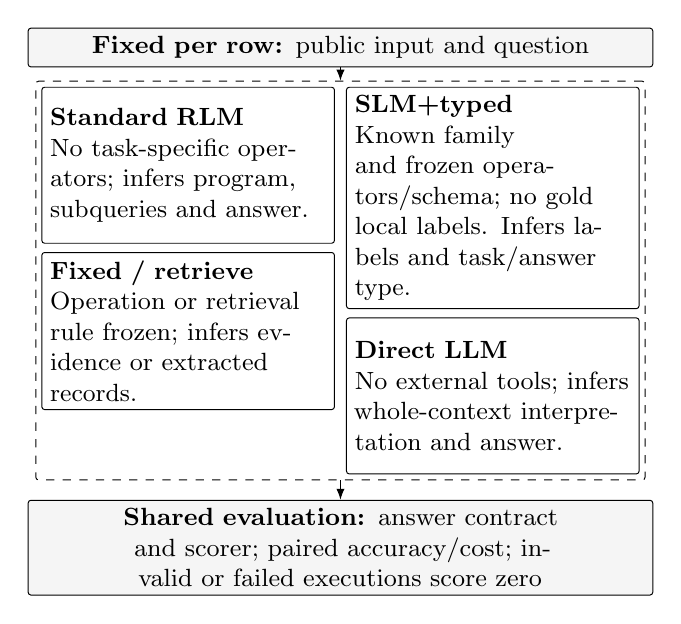
\begin{tikzpicture}[
  font=\small,
  % All four route nodes share one minimum height so both grid rows align.
  % At 0.70in the SLM+typed node outgrew its neighbour and pushed the whole
  % right-hand column 3.6pt below the left, leaving the enclosure lopsided.
  route/.style={draw, rounded corners=1pt, align=left, text width=1.38in,
    minimum height=0.78in, inner sep=3pt, line width=0.35pt},
  shared/.style={draw, rounded corners=1pt, align=center, text width=3.04in,
    inner sep=3pt, fill=black!4, line width=0.35pt},
  flow/.style={-{Latex[length=1.4mm]}, line width=0.4pt}
]
\node[shared] (input) {\textbf{Fixed per row:} public input and question};
\node[route, anchor=north east] (rlm) at ([xshift=-2pt,yshift=-7pt]input.south)
  {\textbf{Standard RLM}\\No task-specific operators; infers program, subqueries and answer.};
\node[route, anchor=north west] (typed) at ([xshift=2pt,yshift=-7pt]input.south)
  {\textbf{SLM+typed}\\Known family and frozen operators/schema; no gold local labels. Infers labels and task/answer type.};
\node[route, below=3pt of rlm] (fixed)
  {\textbf{Fixed / retrieve}\\Operation or retrieval rule frozen; infers evidence or extracted records.};
\node[route, below=3pt of typed] (direct)
  {\textbf{Direct LLM}\\No external tools; infers whole-context interpretation and answer.};
\node[draw, dashed, rounded corners=1pt, fit=(rlm)(typed)(fixed)(direct),
  inner sep=2pt, line width=0.35pt] (routes) {};
\node[shared, below=7pt of routes] (score)
  {\textbf{Shared evaluation:} answer contract and scorer; paired accuracy/cost; invalid or failed executions score zero};
\draw[flow] (input.south) -- (routes.north);
\draw[flow] (routes.south) -- (score.north);
\end{tikzpicture}
\caption{Route-and-contract schematic. Differences in allowed deployment prior knowledge are declared before comparison. The audit does not identify a scaffold-only causal effect or validate an automatic router.}
\label{fig:fairness-contract}
\end{figure}

\paragraph{Protocol and evidence tiers.}
Each headline claim specifies task, baseline and scorer. Controlled families establish mechanisms under identical generators; public Oolong and BrowseComp rows test transfer; LongBench-v2 diagnostics probe context limits, MCQ position, schema rigidity and split overlap. We label each public row as validation, ablation, replication or pilot under its stated contract. An anonymized hash-verified artifact with protocols, scripts, release-safe aggregates, verifiers and a completed reproducibility checklist accompanies submission.

\paragraph{Estimands, scoring and uncertainty.}
For paired routes $r,s$ on $n$ rows, $\widehat{\Delta}_A=n^{-1}\sum_i(Y_{ir}-Y_{is})$ and $\widehat{\Delta}_C=n^{-1}\sum_i(C_{ir}-C_{is})$; failed or invalid executions have $Y=0$. RLM is observed accuracy--cost dominated only when $\widehat{\Delta}_A\leq0$ and $\widehat{\Delta}_C>0$; positive tradeoffs require deployment-specific valuation. Paired accuracy uses McNemar tests (exact for small discordance); $b,c$ denote first-only and second-only correct. Difference intervals use fixed-seed percentile bootstraps with 50,000 paired-row draws for BrowseComp and 5,000 context-window-cluster draws for Oolong. Primary controlled estimands are paired accuracy and captured cost on T-MIXED and standard-unlabeled Oolong. BrowseComp-Plus supplies separate open-search estimates: the original $N{=}80$ manifest is bounded by two-episode completion and post-stop visibility; an attempted-$N{=}49$ endpoint stopped score-blind; an initial replication fixes $N{=}45$ before output; and the strongest prospective endpoint freezes 45 further untouched queries with iterative search and matched decision/time caps, following matched-budget practice \citep{srlm2026}. Failures are incorrect in every fixed denominator. Subgroup, controller and mechanism-probe tests are descriptive; we make no global familywise claim. The equal-cap endpoint applies Holm adjustment over RLM versus BM25, textual decomposition and iterative search. Oolong scores exact matches and accepted relative-frequency substrings, with $0.75^{|\Delta|}$ for numeric near-misses; we report both the binary exact rate and the partial-credit mean score. MCQ predictions are mapped back after answer shuffling. Because Oolong questions can share contexts, uncertainty resamples 72, 73, 32 and 20 clusters for $N{=}120$, SU-150, CD-45 and VC-45. Intervals are conditional on observed executions; a full CD-45 repeat documents rollout sensitivity for that frozen Oolong endpoint.

\paragraph{Cost accounting.}
RLM cost is decomposed into controller generation, child-query execution and final extraction. API totals capture successful completions and are lower bounds where failed calls return no usage. Direct and SLM baselines are single-call unless retrieval-augmented; fixed operators have zero marginal model cost but nonzero engineering cost. At SU-150, unrounded observed API savings are \$0.022040733/case (\$0.022041 rounded), so a hypothetical \$1,000 implementation budget breaks even after $\lceil \$1{,}000/\$0.022040733\rceil=45{,}371$ cases \citep{kapoor2024agentsmatter}. This is an amortization sensitivity, not a labor estimate or TCO. Self-hosted BrowseComp costs use active runtime by route with generation-plus-judge total reported separately. The verifier checks statistics and costs against stored logs.

\section{Results}

\begin{table*}[t]
\centering
\small
\setlength{\tabcolsep}{5pt}
\begin{tabular}{@{}L{2.9cm}L{3.7cm}L{3.2cm}L{6.8cm}@{}}
\toprule
\textbf{Regime} & \textbf{Best non-RLM} & \textbf{Standard RLM} & \textbf{Boundary supported by this row} \\
\midrule
T-STRUCT exact aggregation & Gemma extract + fixed agg.: 100\%, \$0.0002/ex & 96.7\%, \$0.0198/ex & Known exact aggregation: a typed pipeline matches/exceeds RLM at much lower captured deployed-configuration API cost (about 99$\times$ in this cross-model run; still 9.9$\times$ if Gemma extraction is repriced 10$\times$ higher). \\
\addlinespace[3pt]
T-MIXED directional count & Direct Gemini: 28/30, \$0.0223 total & Repaired RLM: 18/30, \$0.1089 total & Same-model direct inference wins on the deterministic current-contract extension; the earlier $N{=}20$ probe isolates finalizer-contract failure. \\
\addlinespace[3pt]
Oolong specialization stress (CD-45; 1k/4k/262k) & Correct-family SLM+typed: 36/45; wrong-family: 2/45 & Same-tools RLM: 31/45 or 29/45; at least 2.3$\times$ costlier & The typed gain requires correct operation knowledge. Supplying the same tools helps free-form RLM but does not match the specialized route under this protocol. \\
\addlinespace[3pt]
Oolong label-provided \mbox{LP-80/LP-150} & Typed ops: 100\% / 97.3\% & RLM: 82.4\% / 84.7\% & RLM is strong under flexible output schemas but gold-label typed operators expose the schema ceiling. \\
\addlinespace[3pt]
Oolong standard-unlabeled (SU-150; VC-45) & SLM-labeler + typed ops: 98/150, \$0.839; unused-source VC-45 35/45, \$0.312 & RLM 68/150, \$4.145; VC-45 28/45, \$1.139 & Five 8k--131k buckets plus pre-output-locked source-corpus transfer: SLM+typed has the best accuracy/cost point; VC-45's exact-rate interval includes zero while its mean-score interval does not. \\
\addlinespace[3pt]
BrowseComp prospective equal-cap ($N{=}45$) & Text: 37/45, \$1.400; iterative: 33/45, \$1.710; BM25: 25/45, \$0.296 & RLM: 31/45, \$9.873 & The earlier RLM--BM25 gain does not transport: no RLM contrast survives Holm correction, and RLM is 5.8--7.1$\times$ costlier than the stronger adaptive routes. \\
\bottomrule
\end{tabular}
\caption{Compact results by evidence tier. LP-80/LP-150 entries are mean/exact; all other percentages are exact. ``Best non-RLM'' is task-specialized; on T-MIXED it prioritizes accuracy. T-STRUCT is a deployed-configuration cost comparison and CD-45 is diagnostic. Equal-cap BrowseComp costs are route-attributed active runtime; the four route totals sum to \$13.279 and adding the interrupted-episode billing lower bound and primary judging gives \$15.015 overall.}
\label{tab:compact-main}
\end{table*}

\paragraph{Known and semantic operations.}
On T-STRUCT, Gemma extracts records and a fixed Python operator performs the aggregation, which is exact by construction, so this row measures extraction success and cost. It reaches 100\% accuracy versus 96.7\% for RLM at about 99$\times$ lower captured deployed-configuration API cost; because both are near ceiling, the result establishes cost dominance only, and supports neither a reliable accuracy difference nor a pure matched-model scaffold-overhead estimate. T-MIXED requires semantic judgments. A matched Gemini ablation separates finalization from semantic error: the legacy count finalizer returns no valid answers while the JSON finalizer returns valid answers on all 20 examples and solves 13. A deterministic current-contract $N{=}30$ extension compares direct Gemini with the repaired RLM finalizer on a frozen stable-hash manifest: direct Gemini solves 28/30 at \$0.0223, repaired RLM solves 18/30 at \$0.1089 (paired exact $b{=}12,c{=}2,p{=}0.0129$) and the repaired path remains about 4.9$\times$ costlier. We treat T-NLP only as an interface diagnostic because no official RLM accuracy run is logged; moreover, the classification target requires categorical labels while the current aggregation scaffold assumes numeric-style answers.

\begin{figure*}[t]
\centering
\includegraphics[width=\textwidth]{fig_task_comparison_submission.pdf}
\caption{Task-conditioned boundary. (a) Descriptive exact rates on standard-input Oolong development data ($N{=}120$; 24 per bucket). Per-cell rates are descriptive; the inferential contrast is the paired cluster-resampled difference reported in the text, not a per-cell interval. (b) Accuracy versus active-runtime cost on the matched-Qwen equal-cap endpoint (filled circles: prospective seed 20; hollow diamonds: same-row post-hoc seed 21; $N{=}45$ each). Whiskers are Wilson intervals; marker area encodes all-row calls (route order RLM/iterative/text/BM25: 476/426/311/42 and 667/276/312/42). No RLM contrast survives Holm correction in either rollout.}
\label{fig:task-comparison-main}
\end{figure*}

\paragraph{Open-search boundary under stronger controls.}
BrowseComp-Plus provides natural open search without a known typed operator and already reports retriever/agent separation and cost analyses; we add operation-matched routes under equal caps on frozen shards. The original frozen $N{=}80$ manifest uses 1,000 documents per query and matched-Qwen routes: standard RLM, BM25 and textual decomposition. It was completed across two disclosed episodes after ranks 1--37 became score-visible. A method-blinded Gemma~4 judge, sharing no model family with any judged route, scores semantic equivalence to the benchmark's gold answer and gives RLM 54/80 (67.5\%), text 48/80 (60.0\%) and BM25 39/80 (48.8\%); only the 18.8-point RLM--BM25 interval excludes zero. A separate GPT-5.6 blind audit likewise supports RLM over BM25 while leaving the RLM--text comparison uncertain.

\emph{Initial fixed-$N$ replication.} We froze 45 rows from a different official query shard with zero overlap against earlier manifests. Model, routes, scorer and failure accounting were unchanged. Gemma~4 scores RLM 33/45 (73.3\%), text 29/45 (64.4\%) and BM25 21/45 (46.7\%). RLM exceeds BM25 by 26.7 points (paired 95\% interval 11.1--44.4; Holm $p{=}0.0151$), while its 8.9-point lead over text is uncertain ($-6.7$--24.4). A blinded GPT-5.6 Sol audit agrees on 128/129 successful outputs ($\kappa{=}0.983$). RLM completes 42/45, costs \$6.746 and has a 425.7-second p95 latency, versus 45/45, \$1.610 and 44.9 seconds for text.

\emph{Prospective equal-cap reversal.} We prospectively froze 45 untouched queries, added iterative lexical search and attempted all 180 Qwen3.6 route cells under common 20-decision/1,200-second caps before semantic scoring, across three disclosed execution episodes; a rank-19 interruption required hash-bound pre-score recovery. RLM scores 31/45 (68.9\%), versus iterative 33/45 (73.3\%), text 37/45 (82.2\%) and BM25 25/45 (55.6\%). Differences are $-4.4$, $-13.3$ and $+13.3$ points, with discordances $6/8$, $5/11$ and $10/4$. Paired 95\% intervals are $[-20.0,11.1]$, $[-31.1,4.4]$ and $[-2.2,28.9]$ points; no contrast survives Holm correction ($p_{\mathrm{Holm}}\geq0.539$). Sol/primary agreement by route is 41/41, 45/45, 45/45 and 41/42 (RLM/iterative/text/BM25; $\kappa{=}0.985$).

RLM completes 41/45 with 50.1/628.8-second median/p95 latency. Iterative/text complete all 45 with 14.1/90.2 and 22.1/47.6 seconds; BM25 completes 42/45. On 39 common completions, scores are 30/28/31/22; this post-treatment sensitivity leaves the adaptive routes near parity. A question-only Qwen leakage probe scores 0/45 under both judges: neither finds a correct answer without the corpus. The earlier RLM--BM25 advantage therefore does not transport; Figure~\ref{fig:task-comparison-main}(b) plots both equal-cap rollouts against active-runtime cost. Open search alone is not a sufficient routing signal.

\emph{Post-hoc seed-21 repeat.} RLM/iterative/text/BM25 complete 37/45, 45/45, 45/45 and 42/45 and score 30/31/29/22; no RLM contrast survives Holm ($p_{\mathrm{Holm}}\geq0.346$). A cap-valid completion finishes within 1,200 seconds: RLM has 36/45, and on 34 rows cap-valid for every route the scores are 28/23/20/18. This post-treatment sensitivity puts RLM first, separating attrition from conditional accuracy. Across four descriptive cross-seed tests, RLM is stable ($b{=}8,c{=}7,p{=}1.0$) while text shifts ($b{=}9,c{=}1,p{=}0.021$); the latter does not survive four-test correction. RLM costs 12.1--15.9$\times$ the adaptive routes. Sol agrees on 166/169 outputs ($\kappa{=}0.961$); the repeat is not pooled with the prospective endpoint.

\emph{Label-provided Oolong.} On LP-80 mean score RLM reaches 82.4\% against 70.0\% for a generic fixed-parser/SLM fallback, although that difference is uncertain ($p{=}0.089$); its largest gain is on timeline questions and deterministic parsing remains perfect on counting. Gold-label typed operators reach 100\% on the same split, so RLM is not the strongest LP-80 route. On frozen held-out LP-150, RLM reaches 84.7\% exact while typed rules fixed before evaluation reach 97.3\% ($b{=}23,c{=}4,p{<}0.001$). Gold local labels make these aggregation/output-schema ablations, not end-to-end Oolong results. They show that RLM handles flexible schemas better than a generic parser but not that open-ended Python is uniquely required when the schema family is known.

\emph{Standard-unlabeled Oolong.} All central public-contract checks use \texttt{context\_window\_text} without gold local labels. An $N{=}120$ development replication established the SLM$>$RLM direction across every 8k--131k bucket (Figure~\ref{fig:task-comparison-main}(a)), with a paired $22.5$-point exact-rate advantage ($b{=}37,c{=}10,p{=}9.8{\times}10^{-5}$; 72-cluster interval $11.9$--$33.0$); the fixed pipeline was then evaluated on SU-150, CD-45 and pre-output-locked VC-45 after one parser repair applied only to rows returning no call, a condition visible without scoring.

On SU-150, SLM+typed solves 98/150 at \$0.839, versus RLM 68/150 at \$4.145 and direct Gemini 65/150 at \$1.939. Discordance favors SLM over RLM ($b{=}44,c{=}14,p{=}1.00{\times}10^{-4}$); no direct--RLM difference is detected ($p{=}0.788$). The 73-cluster interval gives a 10.6--29.9 point SLM advantage but all rows reuse earlier project context windows so SU-150 is scale/method-lock evidence only.

VC-45 removes the known source-corpus overlap: its official validation rows come from \texttt{spam} and \texttt{trec\_coarse}, absent from the test split and every earlier project Oolong artifact. The question parser agrees with metadata on all 45 VC-45 rows; SU-150 and CD-45 carry no equivalent check. SLM+typed solves 35/45 at \$0.312, versus RLM 28/45 at \$1.139 and direct Gemini 23/45 at \$0.658. SLM--RLM discordance is $b{=}10,c{=}3,p{=}0.092$ (Holm $p{=}0.185$); the 20-cluster exact-difference interval is 0.0--31.1 points while the mean-score interval is 3.0--30.9. RLM reaches 13/15 on user questions but 6/15 on counting. Task and source are not factorially balanced, so subgroup differences are descriptive. The specialized route remains cheaper and directionally favored under source-corpus transfer but VC-45 alone establishes neither a significant exact-rate advantage nor document-level independence.

CD-45 retains the specialization controls: wrong-family typing collapses from 36/45 to 2/45 while giving free-form standard RLM the same operator library reaches 31/45 or 29/45 but remains at least 2.3$\times$ costlier. An independent standard-RLM repeat drops from 27/45 to 21/45. Together, SU-150 supplies scale, VC-45 supplies source-corpus transfer and CD-45 isolates specialization and same-tools behavior; none is a full Oolong leaderboard.

\paragraph{Controller and stronger-family boundaries.}
The main Oolong rows use Gemini~2.5 Flash because they evaluate the released standard-RLM stack we could run reproducibly with cost logs. Strict-stop GPT-5 and GPT-5.6 Luna standard-RLM runs on CD-45 reach 23/45 and 26/45; SLM+typed remains higher ($p{=}0.00235$ and $p{=}0.041$). On frozen CD-15, the official trained Qwen policy reaches 10/15 and the project-recorded, frozen-before-execution official-code $\lambda$-RLM row reaches 8/15, versus 15/15 for SLM+typed. The complete $\lambda$ row attempts all IDs on one pinned Qwen3-8B/vLLM deployment and counts two 1,800-second timeouts incorrect. Paired exact outcomes favor SLM+typed ($b{=}7,c{=}0,p{=}0.0156$); no difference is detected against direct Gemini, standard RLM/Gemini or official Qwen (all $p{\geq}0.625$). Across controllers and policies, no sensitivity reverses the SLM+typed ordering; different manifests, denominators and fidelity tiers preclude pooling. These checks show that the Oolong ordering is not specific to Gemini~2.5 Flash but they do not establish official SRLM/$\lambda$-RLM/RAH benchmark parity; the central claim stays on the released standard implementation.

\paragraph{Route recommendation.}
Evidence supports two tiers. When task type is known or reliably inferred from the query, test the cheapest mechanism that matches the operation: fixed operators for exact aggregation, retrieval or semantic workers for matching, SLM/direct calls for local classification and question-parsed typed aggregation for known Oolong-style aggregation families. When no tested typed route captures the request, compare retrieval, textual decomposition and iterative search before treating RLM as a candidate. The Oolong results show that flexible schemas need not require open-ended generated Python; the prospective BrowseComp endpoint shows that open search does not itself justify RLM.

\section{Mechanism Analysis}

Table~\ref{tab:mechanisms} groups qualitative cross-task failure patterns by layer, setting and deployment implication; frequencies are unlabeled.

\begin{table*}[t]
\centering
\small
\setlength{\tabcolsep}{4pt}
\begin{tabular}{@{}L{2.95cm}L{3.9cm}L{4.4cm}L{5.6cm}@{}}
\toprule
\textbf{Mechanism} & \textbf{Where observed} & \textbf{What fails} & \textbf{Paper implication} \\
\midrule
Known exact operator & T-STRUCT aggregation stage, Oolong counting & In the deployed configurations, generated programs add calls without improving accuracy when the symbolic operation is known & On the evaluated known-schema aggregation rows, standard RLM is cost-dominated at the observed operating points by typed extraction plus explicit deterministic code. \\
\addlinespace[3pt]
Final-answer contract sensitivity & T-MIXED matched probe; T-NLP compatibility diagnostic; official-code $\lambda$ row & Older RLM contract produced no finalized answers; two $\lambda$ outputs recover the gold content but violate the answer contract & Convergent evidence from three methods points at the finalization layer; attribution across the whole scaffold is untested. \\
\addlinespace[3pt]
Semantic local judgment & T-MIXED & Regex-like generated programs overfit vocabulary or miss directional meaning & Structured local judgments can beat generated operators; T-MIXED shows direct local judgment beating repaired RLM while costing 4.9$\times$ less. \\
\addlinespace[3pt]
Output-schema rigidity & Oolong timeline/user for generic fp+SLM; question-parsed typed diagnostic & Fixed parser assumes date/numeric outputs while the task requires labels or user IDs & The generic parser fails on flexible schemas; typed operators remove that failure when the schema family is inferable. \\
\addlinespace[3pt]
Open heterogeneous search & BrowseComp-Plus & An initial fixed-$N$ shard favors RLM over BM25, but neither equal-cap rollout yields a Holm-significant RLM contrast; their descriptive route ordering changes while RLM remains costlier & Open search alone does not select RLM; matched decomposition/search, completion and cost-tail controls are required before routing. \\
\addlinespace[3pt]
Context-window constraint & LB2 $>$500k subset & Direct model cannot ingest the full input; retrieval alone can miss distributed evidence & Over-window inputs motivate evaluating RLM or recursive/harness decomposition but benefit over tuned retrieval is not established here. \\
\addlinespace[3pt]
Evaluation-format bias & LB2 multiple choice & Retrieval outputs are sensitive to answer-position priors & MCQ debiasing is a prerequisite before interpreting retrieval-vs.-RLM differences. \\
\bottomrule
\end{tabular}
\caption{Mechanism-level error analysis grouped by layer, setting and deployment implication.}
\label{tab:mechanisms}
\end{table*}

\paragraph{Why LLM+SLM is not automatically superior.}
The evaluation also tests the intuitive alternative "use a strong LLM to orchestrate cheap SLM workers" \citep{narayan2025minions}. This helps when the controller mainly decomposes semantic work but it is not an automatic replacement for deterministic operators. On exact tasks, a controller is unnecessary because the program is known. On T-NLP, LLM+SLM reaches 83.3\%, compared with 87.5\% for SLM direct while costing about 3.4$\times$ more within the evaluated route set. On LB2-style QA, it inherits retrieval and MCQ-bias errors unless the evidence-selection stage is corrected. The viable version is therefore task-conditioned: use LLM+SLM for local interpretation, not for operations already solved by fixed code or retrieval.

\paragraph{Representative trace evidence.}
Table~\ref{tab:trace-vignettes} lists four released CD-45 cases chosen by outcome pattern. Stored T-MIXED traces show successful RLM programs synthesizing dual-gate filters over context slices while observed failures over-broaden vocabulary or depend on brittle final-answer contracts: one false positive counts generic financial "efficiency" language as a cost-reduction event and the matched-model rerun shows the old count contract never finalizes. The repaired JSON contract finalizes every row but still misses seven semantic counts. CD-45 paired examples show the same layered pattern: SLM+typed and direct prompting fix an RLM relation error, both RLM controllers and SLM+typed recover a most-frequent-user row that direct Gemini misses and one SLM failure is a typed tie/normalization edge despite exact local labels. Same-operator RLM failures add wrong routes, malformed answers, tool-use confusion and timeouts. These traces show where the failures surface; on their own they cannot attribute them to the scaffold as a whole.

\begin{table*}[t]
\centering
\small
\setlength{\tabcolsep}{4pt}
\begin{tabular}{@{}L{1.85cm}L{4.85cm}L{4.35cm}L{5.8cm}@{}}
\toprule
\textbf{CD-45 case} & \textbf{Observed outputs or program behavior} & \textbf{Localized failure} & \textbf{What the case establishes} \\
\midrule
912090010 & Gold is ``less common.'' SLM+typed, direct Gemini and GPT-5 RLM are correct; standard RLM/Gemini returns ``same frequency.'' & Relation/count error in one scaffold rollout & The standard-RLM error is not a universal context-understanding failure; both direct and structured routes recover the relation. \\
\addlinespace[3pt]
312030020 & Gold user is 16226. Both RLM controllers and SLM+typed recover it; direct Gemini returns 72294. Same-operator RLM counts user IDs and selects the mode in one iteration. & Direct whole-context aggregation error & RLM can be the useful structured route on an individual aggregation case, even where it is not the strongest aggregate route overall. \\
\addlinespace[3pt]
710070026 & Gold least label is neutral. Standard RLM and direct Gemini are correct; SLM+typed returns contradiction despite 7/7 correct local labels. & Typed tie/normalization edge & Typed pipelines also fail above the local-label layer; the audit is not a one-sided catalogue of RLM errors. \\
\addlinespace[3pt]
410040043 & Convenience same-tools RLM succeeds after 9 iterations, 7 code blocks and 3 tool calls; atomic same-tools RLM uses 16 iterations, 15 blocks and 14 calls but emits a non-matching final form. & Tool-interface confusion and finalization & Supplying the same operators can narrow accuracy differences while retaining substantial orchestration and interface overhead. \\
\bottomrule
\end{tabular}
\caption{Representative released CD-45 traces selected by outcome pattern and reported as illustrations only. The first three cases come from the paired trace exhibit; the fourth comes from the completed same-operator trajectories. Aggregate conclusions remain tied to the full frozen rows.}
\label{tab:trace-vignettes}
\end{table*}

\paragraph{Evaluation-format bias.}
LongBench-v2 Academic QA is multiple-choice so answer-position priors confound retrieval-vs.-RLM comparisons. On the $N{=}50$ discovery set, canonical BM25 predicts A 68\% of the time while gold-A is 18\%. Rotating priming improves pooled $N{=}94$ ($p{=}0.015$) but not held-out $N{=}44$ ($p{=}1.0$); single-call accuracy is unmeasured. We therefore keep it as a validity diagnostic, with prior debiasing comparisons in the supplement.

\section{Related Work}

RLM externalizes context through controller-generated programs and recursive calls \citep{zhang2025rlm}. SRLM questions recursion as the driver, $\lambda$-RLM uses typed functions, LCM moves recursion into deterministic operators and coding agents and recursive harnesses match or exceed RLM on long-context suites \citep{srlm2026,lambdarlm2026,ehrlich2026lcm,cao2026codingagents,lumer2026rah}. Unlike these mechanism studies, we match each family's \emph{operation} on fixed rows and scorer with paired uncertainty. Wang reports model/task-dependent depth, cost, latency and strong-model degradation \citep{wang2026thinkdontoverthink}. We add prospectively locked route comparisons, not a universal family policy.

Cost-aware scaffold evaluation is the closest precedent: simpler baselines can Pareto-dominate agents \citep{kapoor2024agentsmatter}. We extend this evaluation principle to deployment \emph{routes}, contracts and dollars to ask when adaptive programs justify their overhead.

Oolong formulates long-context aggregation as local labeling followed by pooling and includes a labels-provided setting that isolates aggregation from classification \citep{bertsch2025oolong}. We treat label-provided runs as a mechanism ablation and standard-input runs as a costed comparison with standard RLM under the same contract. LongBench-v2 and LongBench Pro cover realistic multitask reasoning \citep{bai2025longbenchv2,longbenchpro2026}; complementary work tests effective context, literal-matching shortcuts and retrieval/routing/length effects \citep{hsieh2024ruler,yen2025helmet,zhang2024infinitebench,nolima2025,li2025lara}. We use LongBench-v2 only as a context-window and multiple-choice diagnostic, not as a broad leaderboard.

Divide-and-conquer, deep-search evaluation and model-routing systems separate evidence selection, tool choice and answer synthesis \citep{xu2026divideconquer,song2026demystifying,ong2024routellm}. We compare them with fixed operators, retrieval, semantic workers, direct inference and standard RLM under logged API costs and explicit evidence grades.

\section{Limitations}

\paragraph{External validity.}
The study diagnoses task-conditional failure modes, not average long-context performance. VC-45 is source-corpus disjoint but not document disjoint because Oolong lacks document IDs; SU-150 reuses windows. Official-family evidence covers CD-15 only. The controlled curve ends at 131k; CD-45 adds 1k/4k/262k stress rows and LB2 $>$500k remains diagnostic.

\paragraph{Measurement.}
Equal-cap evaluation attempts all 180 cells under fixed caps across three disclosed episodes. No human adjudication is available; amid judge fragility \citep{tan2025judgebench}, cross-family agreement and a leakage control test stability, not human validity.

\paragraph{Cost and scope.}
Costs exclude engineering and TCO; alternatives are not exhaustive and recursion depth is fixed. BrowseComp has 45 rows over 1--12 required documents; no subgroup was predeclared and post-hoc bins reach $n{=}10$, so we infer none. BM25 is a lexical floor; a post-hoc same-row Qwen3-Embedding-8B rerank remains below RLM (20/49 vs.\ 35/49, $p{=}0.0026$; supplement) but is not full-corpus dense retrieval. Seven repeat RLM calls exceed the cap and score incorrect. Missing usage requires provider/runtime reconciliation; self-hosted and API dollars remain separate.

\paragraph{Ethics and AI assistance.}
The study uses public or synthetic benchmarks and no human-subject data. AI tools assisted coding, orchestration and editing; analyses, citations, figures and text were human-verified.

\section{Conclusion}

Matched routes lead on known operations; controls show that operation knowledge matters beyond tool access. Across two equal-cap rollouts no RLM contrast survives multiplicity correction while RLM costs 5.8--15.9$\times$ the adaptive alternatives. This supports requiring measured gains rather than assuming a universal routing policy.

\bibliography{../references}

\end{document}
